\documentclass[twoside,11pt]{article}

\usepackage{aa228-jmlr2e}
\usepackage{amsmath}
\usepackage{graphicx}
\usepackage{lipsum}
\usepackage{listings}
\usepackage{url}
\usepackage{cleveref}
\usepackage{subcaption}
\usepackage{tikz}
\usetikzlibrary{calc}

\usepackage{enumitem}

\setlist[itemize]{noitemsep}  % or \setlist[itemize]{itemsep=0pt, topsep=0pt}

\begin{document}

\title{\texttt{trajectory\_utils}: Mathematical background}


%===========================================
\name{Stuart Johnson}
\email{stuart.g.johnson@gmail.com}

\maketitle

\tableofcontents

\section{Cartpoles}

\begin{figure}[h!]
\centering
\begin{minipage}{0.6\textwidth} % adjust width to taste
  \centering
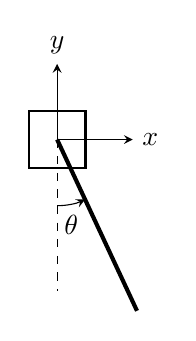
\begin{tikzpicture}[scale=1.2, >=stealth]

  % Parameters
  \def\cartW{0.6}     % cart width
  \def\cartH{0.6}     % cart height
  \def\L{2.0}         % pole length
  \def\thdeg{25}      % pole angle from downward vertical (for illustration)
  \def\roff{0.1}

  % Cart center & pivot
  \coordinate (cartcenter) at (0,0);
  \coordinate (pivot) at ($(cartcenter)+(0,\cartH/2)$);
  \coordinate (poleend) at ($(pivot)+({\L*sin(\thdeg)}, {-\L*cos(\thdeg)})$);

  % Cart (small box)
  \draw[thick]
    ($(cartcenter)+(-\cartW/2,0)$) rectangle
    ($(cartcenter)+(\cartW/2,\cartH)$);

  % Axes from the pivot
  \draw[->] (pivot) -- ++(0.8,0) node[anchor=west] {$x$};
  \draw[->] (pivot) -- ++(0,0.8) node[anchor=south] {$y$};

  % Downward vertical from pivot (reference)
  \draw[dashed] (pivot) -- ++(0,-1.6);

  % Pole: angle measured from negative vertical toward positive x
  % So direction = -90 + \thdeg degrees
  \draw[line width=1.5pt]
    (pivot) -- ++({\L*sin(\thdeg)}, {- \L*cos(\thdeg)});

  % Mark angle theta at pivot (between downward vertical and pole)
  \begin{scope}
    \path (pivot) ++(0,-0.9) coordinate (downref);
    \draw[->]
      (pivot) ++(0,-0.7) arc[start angle=-90,
                             end angle={-90+\thdeg},
                             radius=0.7];
    \node at ($(pivot)+(0.15,-0.9)$) {$\theta$};
   
  \end{scope}
  
  % an attempt at an offset r arrow by gpt5
  
    % ---- r arrow along the pole ----
    % rstart: 10% along the pole from pivot
    % rend:   ~67% along the pole from pivot
    %\coordinate (rstartbase) at ($(pivot)!0.10!(poleend)$);
    %\coordinate (rendbase)   at ($(pivot)!0.67!(poleend)$);
    
    % Offset both points by roff perpendicular to the pole
    %\coordinate (rstart) at ($(rstartbase)!{\roff}!90:(poleend)$);
    %\coordinate (rend)   at ($(rendbase)!{\roff}!90:(poleend)$);

    % Break the arrow in the middle for the label
    %\coordinate (rmid1) at ($(rstart)!0.45!(rend)$);
    %\coordinate (rmid2) at ($(rstart)!0.55!(rend)$);

    % Draw arrow segments along the pole
    %\draw[->, dashed] (rstart) -- (rmid1);
    %\draw[dashed] (rmid2) -- (rend);

    % Label r centered in the gap
    %\node[fill=white, inner sep=1pt] at ($(rstart)!0.5!(rend)$) {$r$};
 

\end{tikzpicture}
\caption{\small Cart–pole system. The cart is actuated by some means and is constrained to move along $\pm x$. Objectives are to swing the pole up to vertical - and/or stabilize it there. The physical cart is actuated by a belt drive, and the pole is a steel rod.}
\label{fig:cartpole-diagram}
\end{minipage}
\end{figure}

\subsection{Equations of motion}

By inspection, figure \ref{fig:cartpole-diagram} offers:

\begin{align}
x_r(t) = r sin\theta(t), r \in [0,L] \\
y_r(t) = - r cos\theta(t), r \in [0,L] \\
\dot{x_r}(t) = r cos\theta(t) \dot{\theta}(t) + \dot{x}(t), r \in [0,L] \\
\dot{y_r}(t) = r sin\theta(t) \dot{\theta}(t), r \in [0,L]
\end{align}

where $r$ parameterizes the location of infinitesimal mass along the pole. It is straightforward to compute the Lagrangian $\mathcal{L} = T - V$ - the first step in deriving the equations of motion.

The kinetic energy $T$ can be written as a sum of the cart kinetic energy and an integral over the pole:

\begin{equation}
T = \int_{r=0}^{r=L} (\dot{x}_r^2 + \dot{y}_r^2) \rho dr + \frac{1}{2} m_c \dot{x}^2
\end{equation}

where $\rho$ is the pole mass per unit length. A bit of algebra yields:

\begin{equation}
T = m_p \frac{L^2}{6} \dot{\theta}^2 + \frac{1}{2}m_p L \cos{\theta} \dot{\theta} \dot{x} + \frac{1}{2} \left(m_p + m_c\right) \dot{x}^2
\end{equation}

where we have used the fact that $\rho L = m_p$.

The (gravitational) potential energy of the cart does not change, so we are left with an integral over the pole:

\begin{equation}
V = g \int_{r=0}^{r=L} y_r \rho dr
\end{equation}

or, equivalently, the potential energy of a mass concentrated at the pole's center of mass:

\begin{equation}
V = - \frac{g m_p L}{2} \cos{\theta}
\end{equation}

Euler-Lagrange now yields two equations:

\begin{equation}
\frac{d}{dt} \left(\frac{\partial \mathcal{L}}{\partial \dot{x}} \right) - \frac{\partial \mathcal{L}}{\partial x} = F_x
\end{equation}

\begin{equation}
\frac{d}{dt} \left(\frac{\partial \mathcal{L}}{\partial \dot{\theta}} \right) - \frac{\partial \mathcal{L}}{\partial \theta} = 0
\end{equation}

The first (force) equation yields:

\begin{equation}
\frac{1}{2} m_p L \left(\cos{\theta} \ddot{\theta} - \sin{\theta} \dot{\theta}^2 \right) + \left( m_p + m_c\right) \ddot{x} = F_x
\end{equation}

and the second (torque) equation yields:

\begin{equation}
\frac{2}{3} L \ddot{\theta} + \cos{\theta} \ddot{x} + g \sin{\theta}  = 0
\end{equation}

or, conveniently:

\begin{equation}
\ddot{\theta} = - \frac{3}{2L} \left( \cos{\theta} \ddot{x} + g \sin{\theta} \right)
\end{equation}

This equation alone can be used to establish an ODE for the cartpole system with the ``velocity'' servo actuation model:

\begin{equation}
\dot{v} = \frac{v_c - v}{\tau}
\end{equation}

or:

\begin{equation}
\ddot{x} = \frac{v_c - \dot{x}}{\tau}
\end{equation}

where $v_c$ is the velocity control. The state ODE for this system is below.

For cart force actuation, we can decouple the above (coupled) equations in $\ddot{\theta}$ and $\ddot{x}$ by thrashing about with some algebra, yielding:


\begin{equation}
\ddot{\theta} = -\frac{6 F_x \cos{\theta} + 6 g \sin{\theta}\left( m_c + m_p \right) + 3 m_p L \sin{\theta}\cos{\theta}\dot{\theta}^2 }{d L}
\end{equation}


\begin{equation}
\ddot{x} = \frac{4 F_x \cos{\theta} + 3 g m_p \sin{\theta}\cos{\theta} + 2 m_p L \sin{\theta}\dot{\theta}^2 }{d}
\end{equation}

where the denominator factor $d$ is:

\begin{equation}
d = 4 m_c + m_p \left(1 + 3 \sin^2{\theta}\right)
\end{equation}

Below we assume the following state space:

\begin{align}
s = 
\begin{bmatrix}
x \\
\theta \\
\dot{x} \\
\dot{\theta} 
\end{bmatrix}
\end{align}


\subsection{Cart force control}

The above equations yield the following first order cartpole system, assuming force control:


\begin{align}
\dot{s} = 
\begin{bmatrix}
\dot{x} \\
\dot{\theta} \\
\ddot{x} \\
\ddot{\theta} 
\end{bmatrix}
=
\begin{bmatrix}
\dot{x} \\
\dot{\theta} \\
\frac{4 F_x \cos{\theta} + 3 g m_p \sin{\theta}\cos{\theta} + 2 m_p L \sin{\theta}\dot{\theta}^2 }{d} \\
-\frac{6 F_x \cos{\theta} + 6 g \sin{\theta}\left( m_c + m_p \right) + 3 m_p L \sin{\theta}\cos{\theta}\dot{\theta}^2 }{d L}
\end{bmatrix}
\end{align}


\subsection{Cart velocity servo control}

For the velocity servo control, we have the simpler (force-free) equations:

\begin{align}
\dot{s} = 
\begin{bmatrix}
\dot{x} \\
\dot{\theta} \\
\ddot{x} \\
\ddot{\theta} 
\end{bmatrix}
=
\begin{bmatrix}
\dot{x} \\
\dot{\theta} \\
\frac{v_c - \dot{x}}{\tau} \\
- \frac{3}{2L} \left(  \frac{v_c - \dot{x}}{\tau} \cos{\theta} + g \sin{\theta} \right)
\end{bmatrix}
\end{align}

\subsection{The \texttt{cvxpy} experience}

\section{Differential Drive Control trajectories}

\subsection{Signed Distance Function (SDF) for obstacle avoidance}

\subsection{Differentiable SDF in pyTorch}

\subsection{The \texttt{cvxpy} experience}

% References
\bibliography{references}


\end{document}

